\chapter{Validation}
\label{ch:VL}

\section{Out-of-Sample and Out-of-Time Validation}
Out-of-sample validation involves evaluating the model's performance on a data set not used during its development. Taking it a step further, out-of-time validation introduces new data covering a more recent time period. The objective is to assess the model's ability to make accurate predictions on unseen data. If the performance metrics differ significantly between in-sample and out-sample data sets, it could signal overfitting. 

The full data set is usually split into a 70\% training and 30\% testing sample. Different ratios, such as 60/40 or 80/20, are also popular choices and mainly depend on the data set size and the number of default events. During the splitting process, it is important to keep the number of default events even in both samples to prevent scenarios where one class is disproportionally larger than the other. This method called stratification reduces the probability of a biased model training and evaluation process.

\section{Model Performance Evaluation}

\subsection{Confusion matrix}
The confusion matrix, illustrated in Figure \ref{fig:vl_confmatr}, is a table comprising four elements, which shows the count of observations correctly (True Positive, True Negative) and incorrectly (False Positive, False Negative) identified cases. A False Positive, denoting a customer predicted to default but survived, is also called Type I Error. A False Negative, where a borrower is expected to survive but defaulted, is also known as Type II error. In practice, a Type II error holds greater severity, as the repercussions of a defaulted exposure outweigh the missed opportunity income from rejecting a non-defaulted application.

\begin{figure}[H]
	\centering
	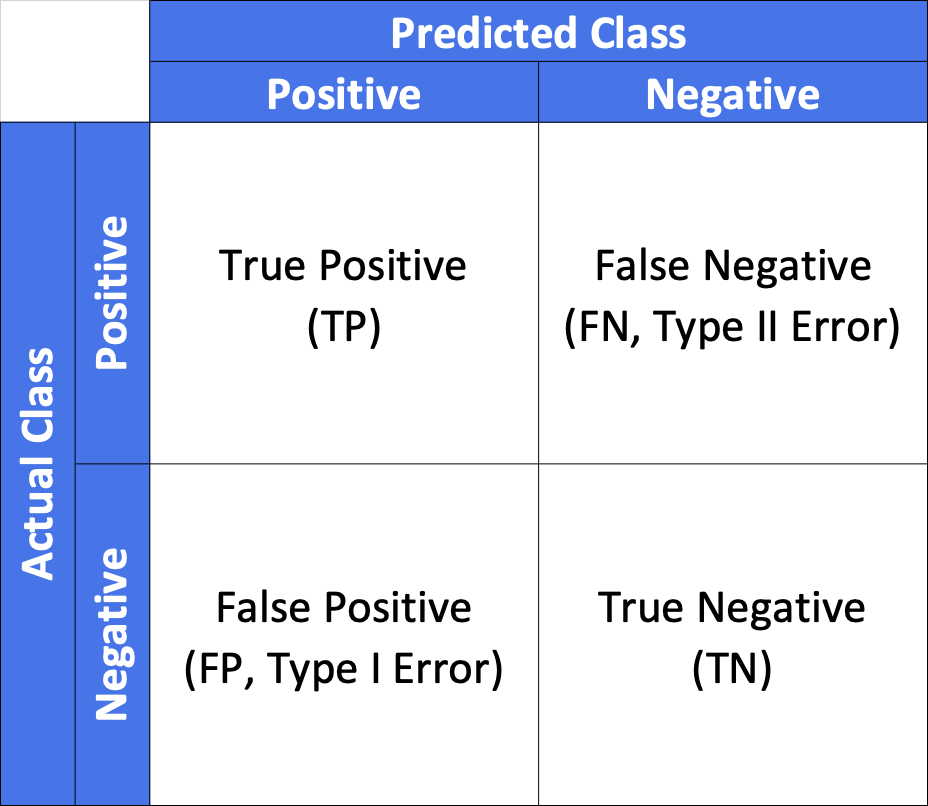
\includegraphics[width=0.45\textwidth]{./VL__confmatrix.png}
    \caption{Confusionmatrix}
    \label{fig:vl_confmatr}
\end{figure}

Using the elements of the confusion matrix, the measures Accuracy, Precision, Recall, F1-Score and others can be calculated, as illustrated in Equations \ref{eq:vl_sens} to \ref{eq:vl_f1}. However, measures like Accuracy and Precision are not recommended for unbalanced data, because they can provide misleading insights about the model's performance. In instances of unbalanced data, a model might attain a high accuracy by simply predicting only the majority class. This high accuracy overshadows the model's ability to identify observations of the minority class correctly. In such scenarios, Recall and F1-score provide a more accurate evaluation of the model's performance. For the transformation from PD to a predicted default flag, a threshold has to be selected. To determine an ideal cut-off, the F1-Score can be utilized, where the value is set where the F1-score attains its maximum.\footnote{\cite{AUC:2023}}

\begin{fleqn}
\begin{flalign} 
\text{Sensitivity} &= \frac{\text{True Positives}}{\text{True Positives} + \text{False Negative}} \\[10pt] \label{eq:vl_sens}
\text{Specificity} &= \frac{\text{True Negative}}{\text{True Negative} + \text{False Positives}} \\[10pt]
\text{Precision} &= \frac{\text{True Positives}}{\text{True Positives} + \text{False Positives}} \\[10pt]
\text{Negative Predictive Value} &= \frac{\text{True Negative}}{\text{True Negative} + \text{False Negative}} \\[10pt]
\text{Accuracy} &= \frac{\text{True Positives} + \text{True Negatives}}{\text{Total Population}} \\[10pt]
\text{Recall} &= \frac{\text{True Positives}}{\text{True Positives} + \text{False Negatives}} \\[10pt]
\text{F1-Score} &= 2 \times \frac{\text{Precision} \times \text{Recall}}{\text{Precision} + \text{Recall}} \label{eq:vl_f1}
\end{flalign}
\end{fleqn}

\subsection{Receiver Operating Characteristic Curve}

The \ac{ROC} Curve, see Figure \ref{fig:vl_roccurve}, is the resulting curve after plotting the proportion of False Positive along the x-axis and the proportion of True Positive along the y-axis. A diagonal line between (0,0) and (0,1) represents the random model, while the perfect model's curve would be a step function that starts at (0,0) straight up and moves horizontally to (1,1). The \ac{AUC} is, as the name suggests, the area below the ROC-curve and the formula for calculating the \ac{AUC} is Equation \ref{eq:vl_auc}.\footnote{\cite{AUC:2023}}

\begin{equation}
AUC = A + \frac{1}{2} \label{eq:vl_auc}
\end{equation}

\subsection{Gini coefficient}
\label{sec:gini}
The Gini coefficient and \ac{AUC} are connected via the given Equation \ref{eq:vl_gini} and a visual presentation is visible in Figure \ref{fig:vl_roccurve}, the areas are designated as A and B. Therefore, they relate the same information but are differently scaled and the Gini coefficient shows an improved interpretability. While the \ac{AUC} has a range between 0.5 (random model) to 1 (perfect model), the Gini coefficient takes on values between 0 (no discriminatory power) and 1 (perfect discriminatory power). In general, the \ac{AUC} can also take on a value below 0.5, but that would indicate that the model's predictions are less accurate than the random model, indicating an issue in the model's ability to differentiate between the classes.\footnote{\cite{AUC:2023}}

\begin{equation}
GINI = \frac{A}{A + B} = \frac{A}{\frac{1}{2}} = (2 * A + 1) - 1 = 2 * \text{AUC} - 1 \label{eq:vl_gini}
\end{equation}

\begin{figure}[H]
	\centering
	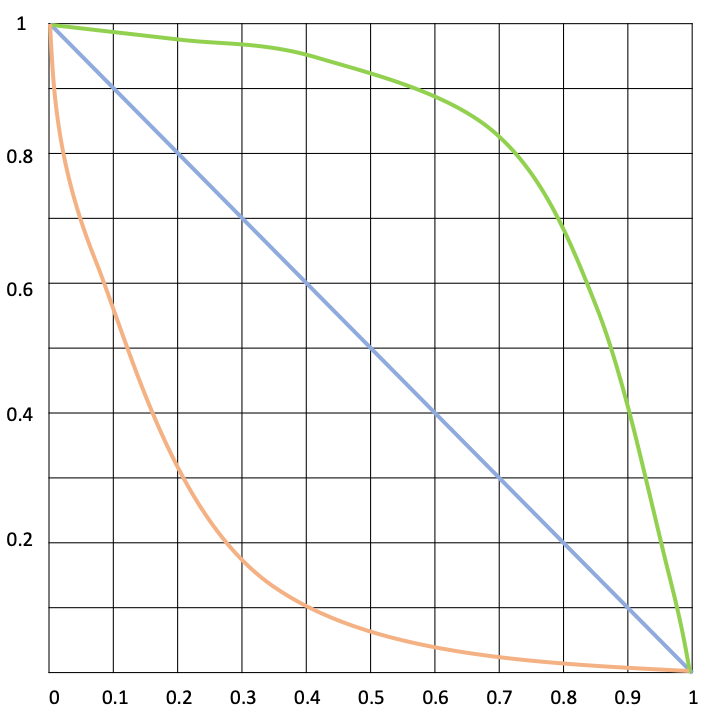
\includegraphics[width=0.5\textwidth]{./VL__ROC_curve.png}
    \caption{AUC-ROC curve}
    \label{fig:vl_roccurve}
\end{figure}

\section{Stability Test}
Stability testing is performed to assess the robustness and consistency of a PD model over time. It examines whether the model's performance remains stable and reliable when applied to data collected at different time periods. Stability testing helps identify potential model deterioration or drift over time, which may be caused by changes in the underlying credit conditions or data characteristics. If significant discrepancies are detected, model recalibration or updates may be necessary to maintain its accuracy and relevance.